
\chapter{Implementation \& Experiments}
In order to evaluate how NEAT can be used to find racing behaviours a number of experiments were conducted. The experiments require a controlled environment which can be reasoned about, and where results can be reproduced. This chapter will cover the implementation of an experiment suite, which includes a racing simulator, an implementation of NEAT, a visualisation system and a control layer which connects the system components. Furthermore, the reasoning behind and execution of the experiments that were conducted will be presented. 



\section{Implementation of the Simulator}
% Givet vårt beteende, hur evaluerar / analyserar vi saker i simulationen. Förklara vår sandlåda / universumet vi skapar.

The simulation is an iterative process where the state of the universe, which only consists of the car and the track, is updated continually. Each update represents a time interval of $10$ milliseconds within the simulated universe. The updates are carried out in direct sequence, thus the simulation rate depends on the clock frequency of the computer running the simulation. However, with the speed of today's computers, multiple updates can be carried out every second. This enables a desktop computer to simulate years of racing in a few hours. 

The simulated car is represented by a simplified model of a real life car. Only the required properties discussed in section \ref{requirements} are simulated. Each update of the car state results in an update of the cars position according to equation \ref{eq:position}

\begin{equation}
    \vec{p}_{n+1} = \vec{p}_{n} + \vec{v}\Delta t 
    \label{eq:position}
\end{equation}

\noindent
Where $\vec{p}_i$ is the position vector of the car in iteration $i$, $\vec{v}$ is the velocity vector of the car and $\Delta t$ is the delta time or the time-step, which is fixed at $10$ milliseconds. This frequency yields a sufficiently high time resolution. At a speed of $100$ m/s, which is slightly higher than the top speed used in the simulator, the car would travel one metre per iteration. In relation to the size of the car and the track, one metre is a short distance.

The velocity vector $\vec{v}$ is updated due to acceleration based on the forces acting on the car. According to classical mechanics, the acceleration $a$ of an object is equal to the applied force $F$, divided by the mass $m$ of the object, a relationship which is described by the equation $F = ma$. This can be extended into higher dimensions by representing the applied force and the acceleration as vectors with one value per axis. Thus the acceleration vector can be found with equation \ref{eq:fma}.

\begin{equation}
    \label{eq:fma}
    \vec{a} = \frac{\vec{F}}{m}  
\end{equation}

\noindent
The car weight used in the simulation is 642 kilogrammes, which albeit being oddly specific, is a reasonable weight for a Formula 1 car without a driver. The rules state that the minimum weight of a car including the driver in full gear but excluding fuel is 702 kilogrammes \cite{f1_weight}. The accelerating force was set to a constant 9100 newton, the braking force 25000 newton and the possible centripetal force 2500 newton.

How much the car is able to turn, or rotate, depends on the current turning radius. The angle the car rotates depends on how far it drives along the circle sector, approximated by $v\Delta t$. As the length of a circle sector is $\theta r$, were $\theta$ is the angle and $r$ the radius of the circle, \(\theta = \frac{vt}{r}\). Combined with equation \ref{equation:turn_radius} the resulting function for the rotation is described in equation \ref{equation:rotation_function}. Skidding of the car is excluded from the simulation as it only represents a state where the traction capabilities have been breached.

\begin{equation}
\label{equation:rotation_function}
    \Delta r = \frac{F_c \Delta t}{mv}
\end{equation}

\noindent
The tracks used in the simulator are flat 3D-meshes with triangle faces. The meshes were modelled in Autodesk Maya and were imported to the simulator in the Wavefront .OBJ format. In order to simplify the representation of the track the cross sections of the track are extracted from the mesh. These cross sections are treated as a series of checkpoints that define the track.  


\section{NEAT Implementation}

NEAT was implemented in C++ primarily based on the descriptions in the original paper \cite{stanley:neat}. Two implementations were also used as references, the latest C++ implementation from the authors themselves \cite{neat_source} and a script written in Lua used in a Super Mario bot \cite{mario_source}. 

In order to verify the implementation of the algorithm it was tested by training it to approximate the logical exclusive-or function (XOR). The reason that the XOR-function is relevant to test is because it is not linearly separable, this means that a neural network requires hidden nodes in order to approximate the function \cite{haykin, stanley:neat}. The test was used to validate that the implementation of the algorithm made additions and changes to the network structure. 

Worth noting is that the neural networks used by NEAT differs slightly from the classical approach. Instead of treating the biases as a separate set of values, a bias input is introduced. The bias input is set to a constant non-zero value. In order to add a bias value to a neuron a connection from the bias input to that node can be added. The bias value of the node can be changed by modifying the connection weight. This is a convenient approach since it allows the algorithm to modify the bias values with the same operations that are used to modify the network topology.

% Ta upp skilnaden mellan NEAT och fs-NEAT?
Additionally, some minor utility features were added to our implementation in order to allow for a more flexible training process. For example, the activation function used in the neural networks is specified as a lambda-function, thus it can be changed at run-time. Therefore, specific activation functions could be used for a specific experiment. Furthermore, the ability to toggle the creation of an initial structure for new networks was added. If the option is enabled, the genomes start with a lattice of connections that connect each input to each output with a randomised weight.
The variant of the algorithm where the initial structure is omitted is called FS-NEAT \cite{whiteson}.

\subsection{NEAT Configuration}
NEAT can be configured in order to change the general behaviour of the algorithm. The configuration used during the project can be found in appendix \ref{appendix:project_settings:neat_constants}. This configuration is based on the Super Mario bot implementation \cite{mario_source} as well as the original paper \cite{stanley:neat}. However, some modifications were performed in order to achieve a more appropriate behaviour.

It was noted that the amount of nodes produced by NEAT was significantly larger than required. Nodes were produced when a simple connection weight modification would have been more appropriate. To prevent this behaviour, the probability of adding a node was decreased.

When performing long training sessions, it also seemed reasonable that allowing networks to stay alive for longer periods of time would be beneficial. This could allow behaviours that initially are non-optimal to prove themselves superior when allowed more time to evolve. Thus the allowed time for a network to live on, before it is killed off by stagnation, was increased.



\section{Training Process}
% Hur går vi till väga för att träna en AI, hur är AI och träning kopplat till resten av systemet
% Hur ser träningen ut:
    % AIn styr bilen i varje simulation step
    % Indata, förklara inte vilken typ av indata, säg bara vart den kommer ifrån.
    % Slutgiltliga resultatet av simulationen ger feedback
The training process adapts neural networks to drive a car. NEAT is utilised in combination with the simulator to train the genomes. The actual learning, i.e. changes to the genomes, is performed by NEAT. However, the evolutionary process requires a measurement of fitness to evaluate genomes. Thus the training procedure is responsible for calculating the fitness of every genome, so that the evolutionary process can proceed. 

In order for the training process to evaluate a genome and calculate its fitness, the simulator is utilised. Calculating the fitness requires information about how well a specific genome has performed. The training process generates a network based on the genome that is about to be evaluated, and provides it to the simulator. The simulator uses this network to control the car during the simulation. In each update of the simulation, the simulator feeds data about the car and its environment into the network, with which the network calculates how to control the car. Once the simulation terminates, the simulator presents the training process with a result that can be used to calculate the fitness.

The following subsections cover the network inputs and outputs used in detail. Furthermore, the evaluation process and fitness function will be covered. 

\subsection{Interpretation}
\label{method:interpretation}
% Talk about how the environment is represented in relation to the neural network.
% How does the AI see the world? What does the inputs look like?
% What kind of output does the AI give to steer and control the vehicle?
% NOTE: Explain the potential solutions, but do not give away which one is being used in the final version, this conclusion needs to come from performing experiments and should thus be presented in the discussion & results.
% Problem modelling. 
% used indata:
% bias
% distance to middle
% distance to left edge
% distance to right edge
% angle to track/mid line
% speed of car 
% corner data, points at [m]:
% 	10
% 	24
% 	42
% 	66
% 	100
% 	144
% 	205
% 	287
% 	397
% 	546
% sums of corner points:
% 	Segment 1, point 1-4, 10-66m
% 	Segment 2, point 4-7, 66-205m
% 	Segment 3, point 7-10, 205-546m

The system requires information about the car and environment in order to decide how to act. Providing the appropriate information, is essential if the system is to learn an effective behaviour. The appropriateness of information depends on the problem and target behaviour. 

The inputs used within the project aim to give an easy way for the system to couple situations with an appropriate action. The input values are summarised in table \ref{tab:input_table} and can be divided into two groups; one that describes the shape of the track in front of the car, and one that describes the current state of the car. Even though not all inputs were used in every experiment, they are all present in at least one experiment each.

\begin{table}[h!] 
  \centering
  \begin{tabular}{ll}
    \toprule
    Name & Description\\
    \midrule
    Track curvature & 10 angles describing the curvature of the track. \\
    Sum of curvature & Three sums of track curvature, angles 1-4, 4-7 and 7-10\\
    \midrule
    Car speed & The current speed of the car\\
    Angle to mid line & Angle between the car direction and the track mid line\\
    Dist. to middle & Distance between the car and the track mid line\\
    Dist. to left edge & Distance between the car and the left edge of the track\\
    Dist. to right edge & Distance between the car and the right edge of the track\\
    \midrule
    Bias & The value 1 to be used as a constant base value in neurons\\
    \bottomrule
  \end{tabular}
  \caption{List of all available inputs for the neural network.}
  \label{tab:input_table}
\end{table}

\begin{wraptable}{r}{0.3\textwidth}
    \hspace{5pt}
    \begin{tabular}{ll}
    \toprule
    Point & Distance [m]\\
    \midrule
    1 & 10\\
    2 & 24\\
    3 & 42\\
    4 & 66\\
    5 & 100\\
    6 & 144\\
    7 & 205\\
    8 & 287\\
    9 & 397\\
    10 & 546\\
    \bottomrule
    \end{tabular}
    \caption{Distance from the car to each point as given input.}
    \label{tab:point_layout}
\end{wraptable}

\noindent
There are two types of input values describing the shape of the track in front of the car. These inputs aim towards letting the system plan ahead for the car, in order to adjust position of the car before arriving at corners. 

The first type is the curvature data, which is a series of angles. The angles are based on the position of the car and 10 points on the mid line of the track. The first angle is calculated from the direction that the car faces and the direction to the first point. The rest of the angles are calculated by comparing the directions of the succeeding line segments defined by the previous points.

The distance between the points increase exponentially for each point. This leads to higher resolution closer to the car where detail is more important, and lower resolution where the general outline of the track is sufficient. For the experiments conducted, an increase of $35\%$ was deemed sufficient with points spanning from 10 meters to 546 meters in front of the car, with the spread presented in table \ref{tab:point_layout}. This distribution of points would give the car the chance to interpret the curvature even further than necessary to plan ahead.

%If not table
%The 

%Pre opponation
%The first type is the curvature data, which is a series of angles. The angles are based on the position of the car and 10 points on the mid line of the track. The first angle is calculated from the direction that the car faces and the direction to the first point. The rest of the angles are calculated by comparing the directions of the succeeding line segments defined by the previous points. The distance between the points increase exponentially by 35 percent for each point. The points are distanced from the car by 10, 24, 42, 66, 100, 144, 205, 287, 397, and 546 metres. The exponential increase of distances makes the resolution higher close to the car where detail is most important, and less resolution where the general tendency is sufficient.

The second type is the summed curvature of three different regions. The regions consist of the points 1 through 4, 4 through 7, and 7 through 10. These summations provide a better overview of the track shape than the individual angles. 

The set of inputs that describe the current status of the car are more simple in nature. They aim towards giving the system the capability of keeping the car on the track at all times. These inputs consist of current car speed measured in meters per second, angle between the cars current direction and the mid line of the track, distance from the car to the tracks mid line, as well as the distance between the car and the left and right edge of the track.

Additionally, a bias value is introduced as an input to the network. The value of this input will always be 1. This is due to the fact that if all inputs to a specific neuron are zero, the neuron would not be able to produce a signal. Since the output of a neuron is the weighted sum of all its inputs, the bias can be used to produce a base value for the sum. 

\begin{table}[h!] 
  \centering
  \begin{tabular}{ll}
    \toprule
    Name & Description\\
    \midrule
    Turning rate & Current steering applied to the car \\
    Acceleration \& braking & Amount of acceleration/braking applied to the car \\
    \bottomrule
  \end{tabular}
  \caption{List of all available outputs for the neural network.}
  \label{tab:output_table}
\end{table}

\noindent
The number output values for the networks used during the project are limited to two. One for turning rate and one for acceleration and braking. An activation function was chosen such that both output values can span from $[-1,1]$. Specifically, the activation function seen in equation \ref{method:activation_function} was chosen.

\begin{equation}
\label{method:activation_function}
    S(t) = \frac{2}{1 + e^{-t}} - 1
\end{equation}

\noindent
For turning rate negative values represents steering right and positive ones to the left. If the output value of a network exceeds the amount of steering that can be applied at the current car speed, the simulator floors the value to that maximum.

For acceleration and braking, a negative value represents braking, while a positive value represents accelerating. The value is interpreted by the simulator as the ratio between the desired and the maximum value, thus a value of $1.0$ correlates to the maximum amount of acceleration.

% The values for turning rate are in the range $[-1,1]$, where negative values represents steering right and positive ones to the left. If the output value of a network exceeds the amount of steering that can be applied at the current car speed, the simulator floors the value to that maximum. For the acceleration and braking, the output values ranges from $[-1, 1]$, where positive values represent accelerating and negative values braking. The value is interpreted by the simulator as the ratio between the desired and the maximum value, thus a value of $1.0$ correlates to the maximum amount of acceleration.

\subsection{Evaluation}
%In order to evaluate the performance of a genome, a fitness value has to be calculated. This is done by building a network from the genome representation and using it as a controller for the car in the simulation. The simulation is then run until either the car has finished the track, crashed, or do not progress. 

%When calculating the fitness, two values from the simulation are considered; the distance progressed on the track and the time spent before termination. Considering both of them in a good way is crucial in order to reward desired behaviour. 

When calculating the fitness, two values from the simulation are considered; the distance progressed on the track and the time spent before termination. Since the evolution of the genomes happen gradually, the performance must also be allowed to progress gradually. Rewarding for distance driven gives an incentive to complete the track and not crash. Time is needed as it distinguishes cars that reach the same distance. After some level of basic improvements in time, advanced racing behaviours will be required to improve further. 

However, if time is valued in combination with progression it might incite to drive fast and crash instead of progressing in distance. One way to solve this is to only consider time it manages to finish the track. In that way, fitness is first rewarded for the progression on the track and then, if the car also completed the track, extra fitness is added for how little time was spent.

As of this, the time contribution to the fitness function is always positive. In addition, as time get smaller it will get increasingly difficult to decrease it further. It may therefore be beneficial if the resolution of the fitness function is greater for smaller time values. One function that satisfies these conditions is \((\sqrt{t_{max}} - \sqrt{t})^2\) presented in figure \ref{figure:time_fitness}, where $t$ is the termination time of the simulation and $t_{max}$ is a suitable upper limit for the track. Combined with distance, the resulting fitness function is as described in equation \ref{eq:fitness_distance_time}.


\begin{figure}
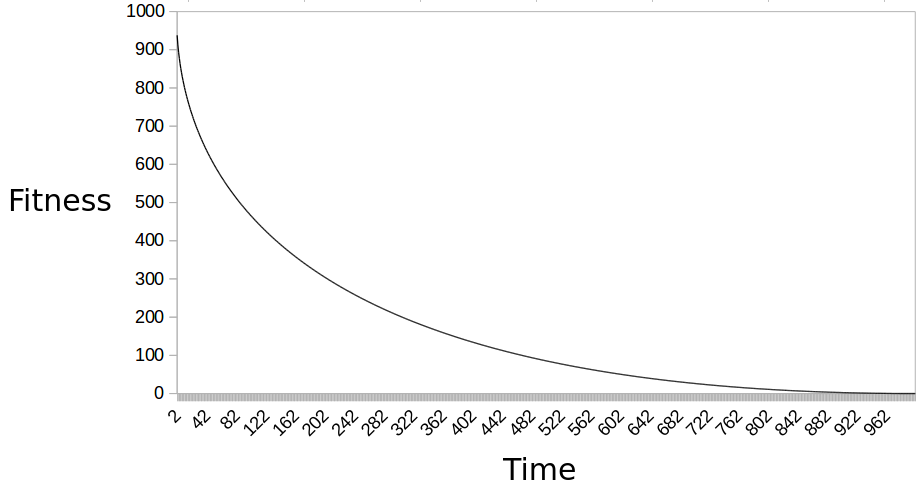
\includegraphics[width=13cm]{fitness_time}
\caption{Example use of the time contribution in the fitness function with $t_{max} = 1000$. The fitness decreases with time, as well as the resolution of the function.}
\label{figure:time_fitness}
\centering
\end{figure}

\begin{equation}
\label{eq:fitness_distance_time}
  f(d, t) =
  \begin{cases}
    d    & \qquad \text{if } d < d_{max} \text{ or } t \geq t_{max} \\
    d_{max} + \lambda*(\sqrt{t_{max}} - \sqrt{t})^2 & \qquad \text{else} \\
  \end{cases}
\end{equation}

\noindent
%Equation \ref{eq:fitness_distance_time} presents the fitness function that was used to evaluate genomes, 
Where the distance driven along the track is denoted by $d$ and the distance to complete a lap is denoted by $d_{max}$. In order to properly balance the importance of lap time and distance driven, the constant $\lambda$ was introduced. During the following experiments, $\lambda=5$ was found to be reasonable constant.

%The function aims towards letting the system learn one task at a time. This should reduce complexity of performing a lap, since the system only has to consider distance driven initially.

It is important to note that the distance driven $d$ is the distance that the car has driven along the track. This distance is equal to the position of the car, projected on the mid line of the track. Thus driving in a sinusoidal pattern will not affect the final distance driven.


\section{Experiments}
The project was an iterative process. Progress was made by experimentation, where different ways to model the problem and train the AI were tried out. In order to establish which aspects of the target behaviour that can be found with NEAT, a number of experiments of varying complexity were conducted. The following subsections will motivate the need for the different experiments and explain how they were conducted.

\subsection{Steering a Car Moving at a Constant Speed}
\label{method:constant_speed}
Driving a car is a complex problem, consisting of several sub-problems. This experiment aims to reduce the problem to one of its components, the steering. Instead of learning to control every aspect of the car, the AI will learn to steer a car that travels forward at a constant speed. The speed is sufficiently low to allow the car to steer through every corner on the circuit. 

The track can be seen in figure \ref{fig:normal_track}. The corners are designed to have an increasing complexity along the track, and consists of a variety of corners. The input points shown in table \ref{tab:point_layout} on page \pageref{tab:point_layout}, covers approximately the two closest upcoming corners, regardless of what section the car is located in.

\begin{figure}[H]
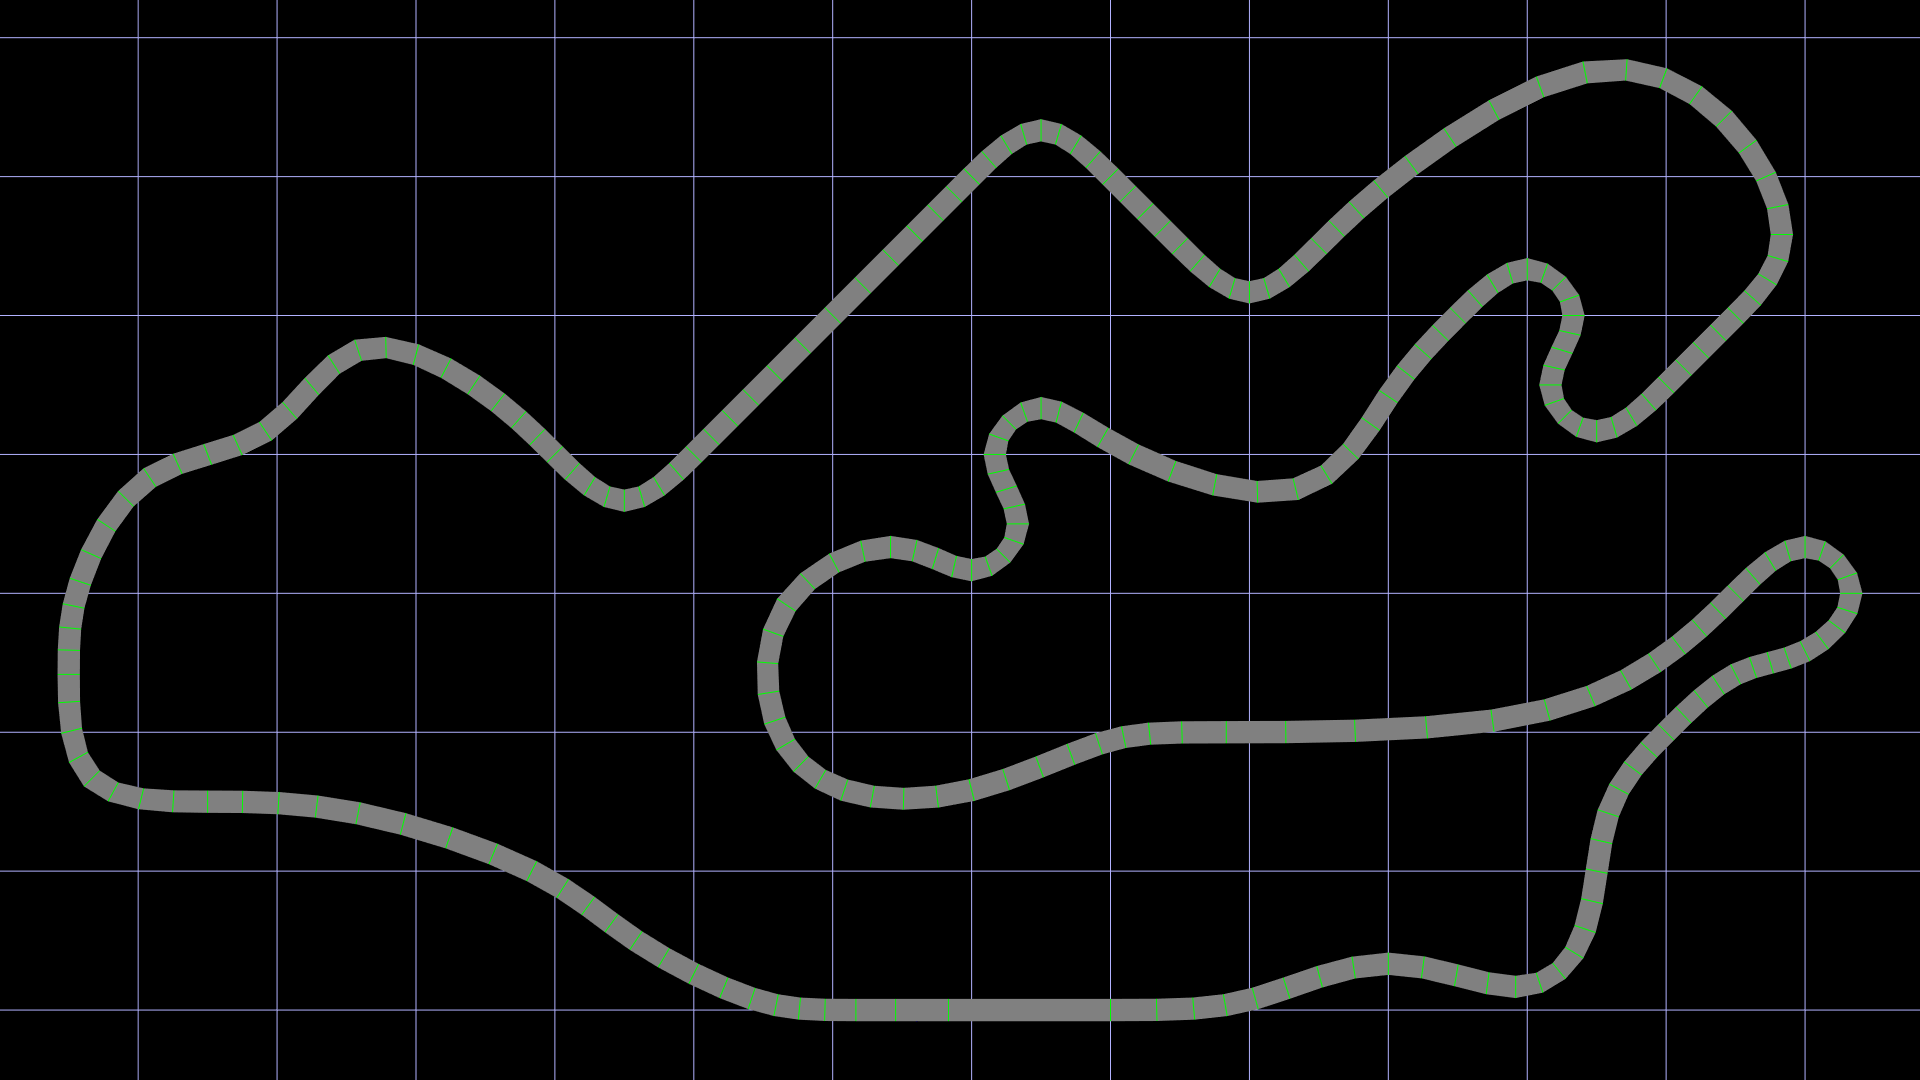
\includegraphics[width=\textwidth]{normal_track}
\caption{Circuit used in constant speed and full control experiment}
\label{fig:normal_track}
\centering
\end{figure}

Two variations of this experiment were conducted at several car speeds. In the first variant, the system learns to steer but is only given local perception of the environment, which in this case means that the car knows its position and orientation relative to the road. In the second variant the number of inputs is increased and the car is given the curve data. Thus the car receives information about the shape of the track ahead.

These experiments will give insight into how well the AI can interpret the provided data and how an increased perception of the track shape affect the behaviour. If the AI successfully learns to steer the car it would ensure that such behaviours can be found with NEAT. Furthermore, it would show which of the provided inputs that are relevant to solving the problem. If the AI learns to steer only using a subset of the inputs, it shows that the other inputs are superfluous. 

% TODO: Formulera om: Without any curvature information, the AI is unable to plan ahead.
% Det känns som en slutsats, det borde kännas mer som det är logiskt sjävklart.
Comparing the result of the different experiment variants should show whether or not the addition of curve data will enable the AI to plan ahead and how that affects the behaviour of the AI. Without any curvature information, the AI is unable to plan ahead. Since it is only aware of the current position and orientation of the car, it is only able to react to that information. It seems reasonable that providing information describing the shape of the track ahead of the car will give the car the chance to plan ahead. Thus improving the AI's ability to take difficult corners and steer effectively. 

% Stuff that could be included in the text above:
% 1. It should also help with deciding whether or not the way in which the track and steering actions are represented needs to be modified in any way, in order to increase network performance.
% 2. When gradually incrementing the speed, what kind of race line do we want the car to perform?

% BAKA IN
%In order to allow the network to plan ahead, a set of new inputs to the network was introduced. The concept of curve data, as explained in section 3.4.1 was provided to the network. Initially, the distance ahead covered by the new input data was 100 meters, but it was later expanded to 300 meters and 500 meters. Other than this change in input data, the inputs and outputs of the network were the same as in the fixed speed experiment.

% Examining this will present relevant information regarding what to expect once the complexity of the problem is increased. It should also help with deciding whether or not the way in which the track and steering actions are represented needs to be modified in any way, in order to increase network performance.

% TODO: Rewrite this once Training Process -> Interpretation has been written, so that we can refer back to that section. 
%The input data to the neural network in this experiment consists of the angle between the car and the mid line, curve data and the sum of the curve data absolute values as well as the current distance from the car to the mid line. The output that is produced by the network is an evenly distributed float value that ranges from $-1$ to $1$, representing full steering to the right and left respectively.

%In order to further increase the complexity of the problem and to examine the possibility of the AI to calculate an optimal race line, the aspect of planning ahead was introduced. The constant speed of the car was increased to a level were going around certain corners in the middle of the track, would not be possible. Thus forcing the network to position the car on a race line that has a larger radius than driving in the middle of the track. Performing this experiment should give some insight into the capabilities of the AI with regards to modifying race lines in order to take a complete lap. Even though the AI might not be able to take the most optimal route, seeing the capabilities of the race line modification could present some interesting information about potential problems or modifications needed.


\subsection{Full Control of the Car}
\label{method:baseline}
In this experiment, the AI will train on driving with full control of the car. In addition to steering it will also control the speed by accelerating and braking. In addition to the position, orientation, and curvature data the AI will be provided with the current speed of the car. The result of the experiment will further establish the limits of the training system. 

Several experiment variations with this configuration will be carried out. In the first variant, which is the baseline experiment, the AI will drive on the same complete circuit as used in the constant speed experiments. This will show whether or not the AI is able to stay on the track to the same extent as when it only steers. Furthermore, it will show whether or not the system can learn to manage the speed in an effective way. If the system is able to find an effective behaviour, the natural response would be to even further increase the complexity of the problem. However, if no effective behaviour is found, it indicates that the training process and system configuration are suboptimal. 

\subsection{Short Track Segments}
\label{subsec:shorttracksegment}
This variant of the experiment will test the system on shorter track segments, only containing one corner each. The motivation for testing short tracks is that it should be easier for the system to find effective behaviours on a short segment than on a complete circuit. This is because the behaviour required to complete a long circuit is generally more complex than the behaviour needed to complete just one corner. Thus, the algorithm will be able to start optimising for speed earlier and on less developed genomes. 

The tracks consist of two straights connected by a corner, and can be seen in figure \ref{fig:short_tracks}. The straights are between $400$ and $500$ metres long and there are three types of corners used. The first corner is a 30-degree corner throughout which the car should be able to keep a high speed. The second one is a 90-degree corner with a small inner radius. The third corner used is a hairpin corner which turns 180-degrees with a small inner radius. 

\begin{figure}[H]
    \centering
    \subfloat[30-degree corner.]{{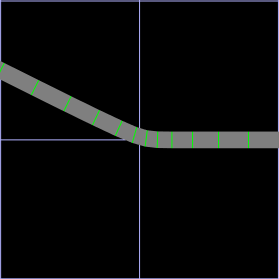
\includegraphics[width=0.28\textwidth]{corner_30}}}%
    \qquad
    \subfloat[Tight 90-degree corner.]{{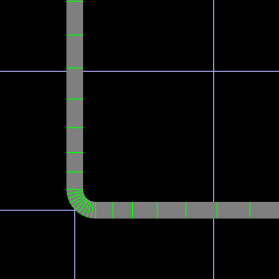
\includegraphics[width=0.28\textwidth]{corner_90}}}%
    \qquad
    \subfloat[180-degree hairpin corner.]{{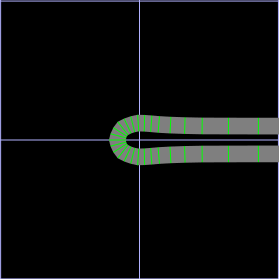
\includegraphics[width=0.28\textwidth]{corner_180}}}%

    \caption{Short track segments with different corner types. The grey line is the track.}
    \label{fig:short_tracks}
\end{figure}

\noindent
Successful results in these experiments would confirm that the system can find effective behaviours for shorter track segments. If that is the case the training process for the short track segments could be extended to solve more complex problems. A scenario where the experiment yield significantly more effective behaviours than the baseline experiment would give insight into the limits of the training process, and how the fitness function is used. This insight could be used to find effective behaviours for longer tracks. 

%==================================================================
%\subsection{Multiple short track segments}

%If the system finds effective behaviours on the short track segments, one interesting experiment is to train one population of genomes on multiple short segments. Finding behaviours effective at several different types of corners is one step towards a more general effective behaviour. Training on multiple track segments could be a safer training environment for the genomes because the consequences of failing on one segment is not necessarily catastrophic. A change that would increase the effectiveness over one segment but leads to a crash on another would be catastrophic on the circuit. However, if the genomes are evaluated on several track segment, failures on one segment can be compensated for by performing well on others. 

%The track segments used are the same ones as in the short track segment experiment, seen in figure \ref{fig:short_tracks}, with the addition of the mirrored versions of those segments. Thus the fitness of a genome is evaluated by summing the fitness acquired on each of the six tracks.

%This experiment could answer three interesting questions. Is the system able to find behaviours effective in multiple scenarios? How does it differ to training different corners in a sequence in a single track? Additionally, how general would that behaviour be? Answers to these questions could give insight into how large the set of training scenarios required to find a fully general behaviour is. 
%====================================================================

%% SKRIV OM ALTERNATING TRACKS IFALL VI SKALL DET
%It will also be tested to alternate which of the track segments are used for the evaluation. Will this let networks progress further, since a temporary decline in some curves will not be noticed? 

\subsection{Mirrored Track}
\label{method:mirror}
One of the project goals is to find generalised behaviour of how to drive in a racing domain. This means that a genome learns to drive regardless of what track it drives on. Instead of finding behaviours effective on a specific circuit, the goal is to find a behaviour that is effective on any circuit. In order to test this a population of genomes is trained on the complete circuit used in previous experiments. Eventually the population will have adapted to the circuit. The population is then transferred to a new circuit, which as shown in figure \ref{fig:mirrored_tracks} is a mirrored version of the one used earlier. This means that the genomes will drive on a track where each corner on the circuit has the same shape but opposite direction of the ones on the other circuit. The development of this population can then be compared to the development of a control group that is only trained on the mirrored track. Note that the number of tests and variation in environment is not enough to prove generality. However, the results will indicate whether or not some degree of generality is obtainable. 

\begin{figure}[H]
    \centering
    \subfloat[The original circuit.]{{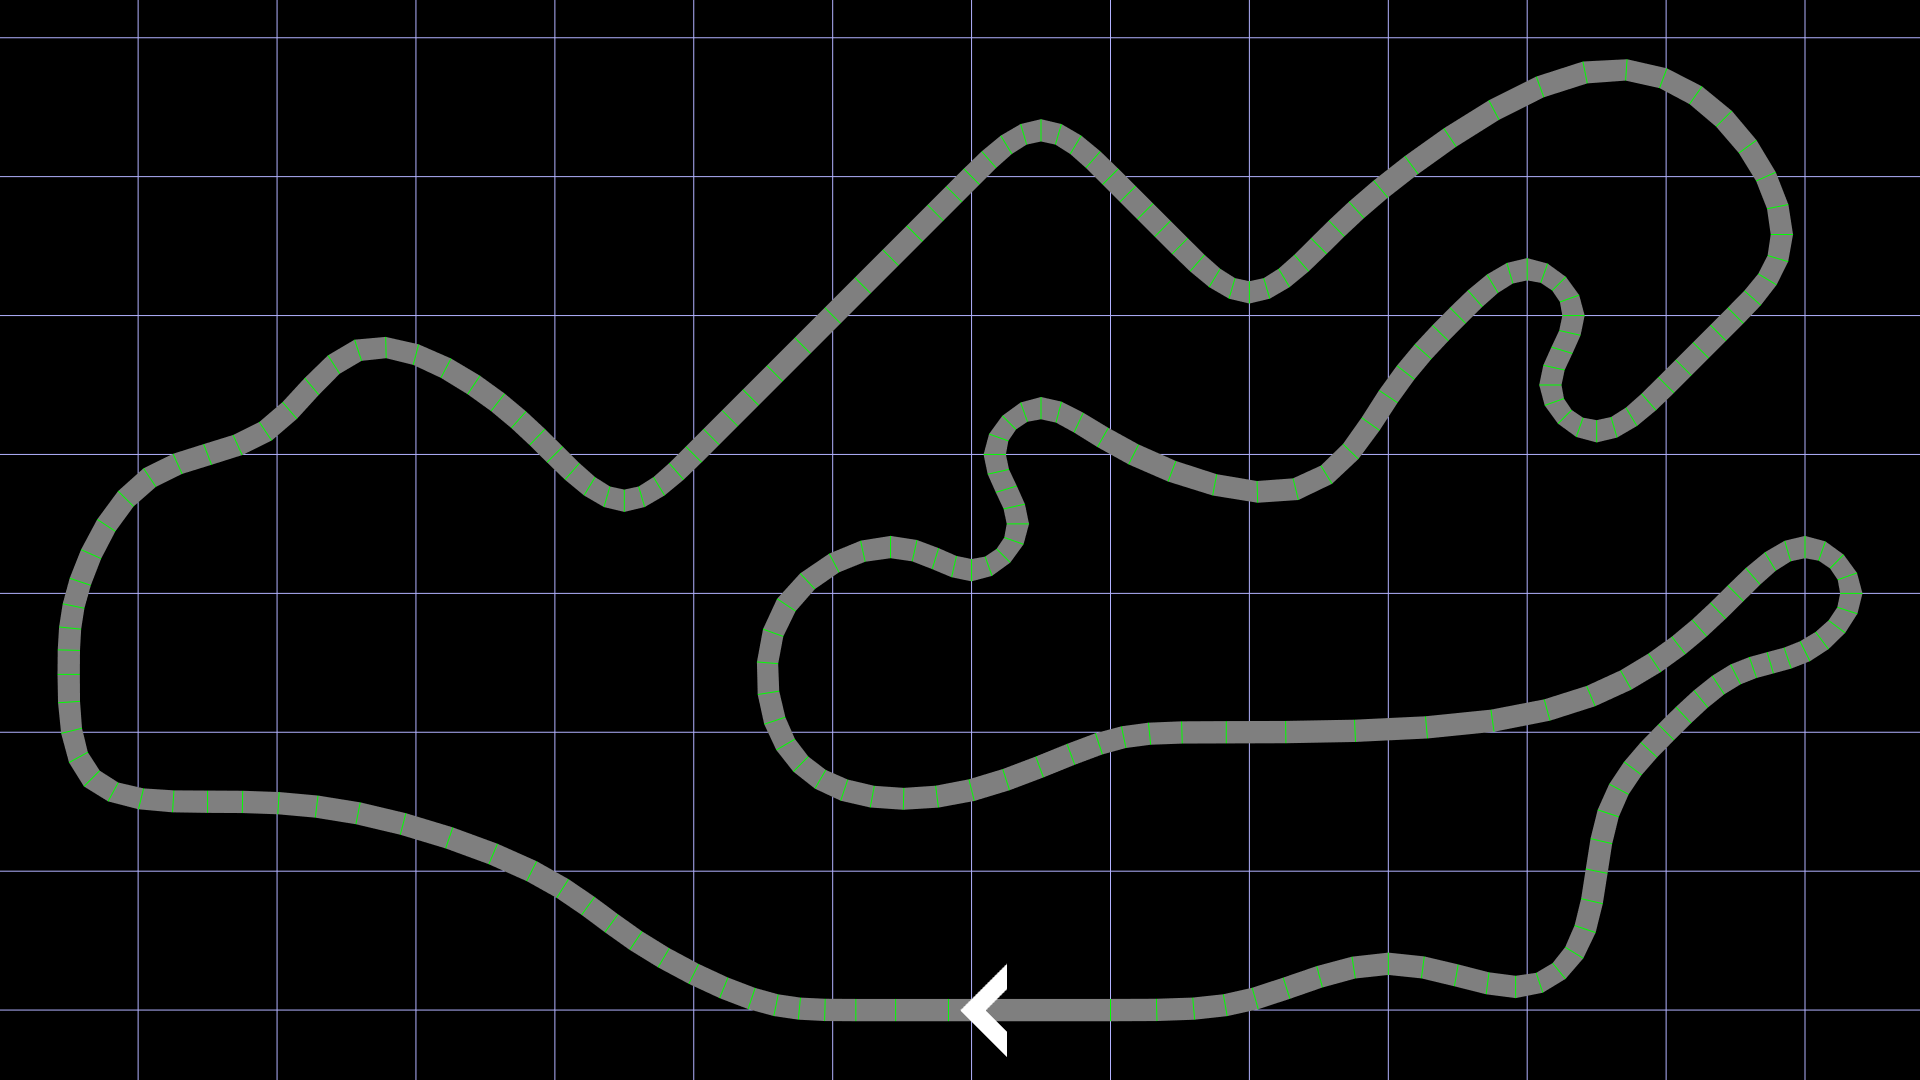
\includegraphics[width=0.45\textwidth]{normal}}}%
    \qquad
    \subfloat[The mirrored circuit.]{{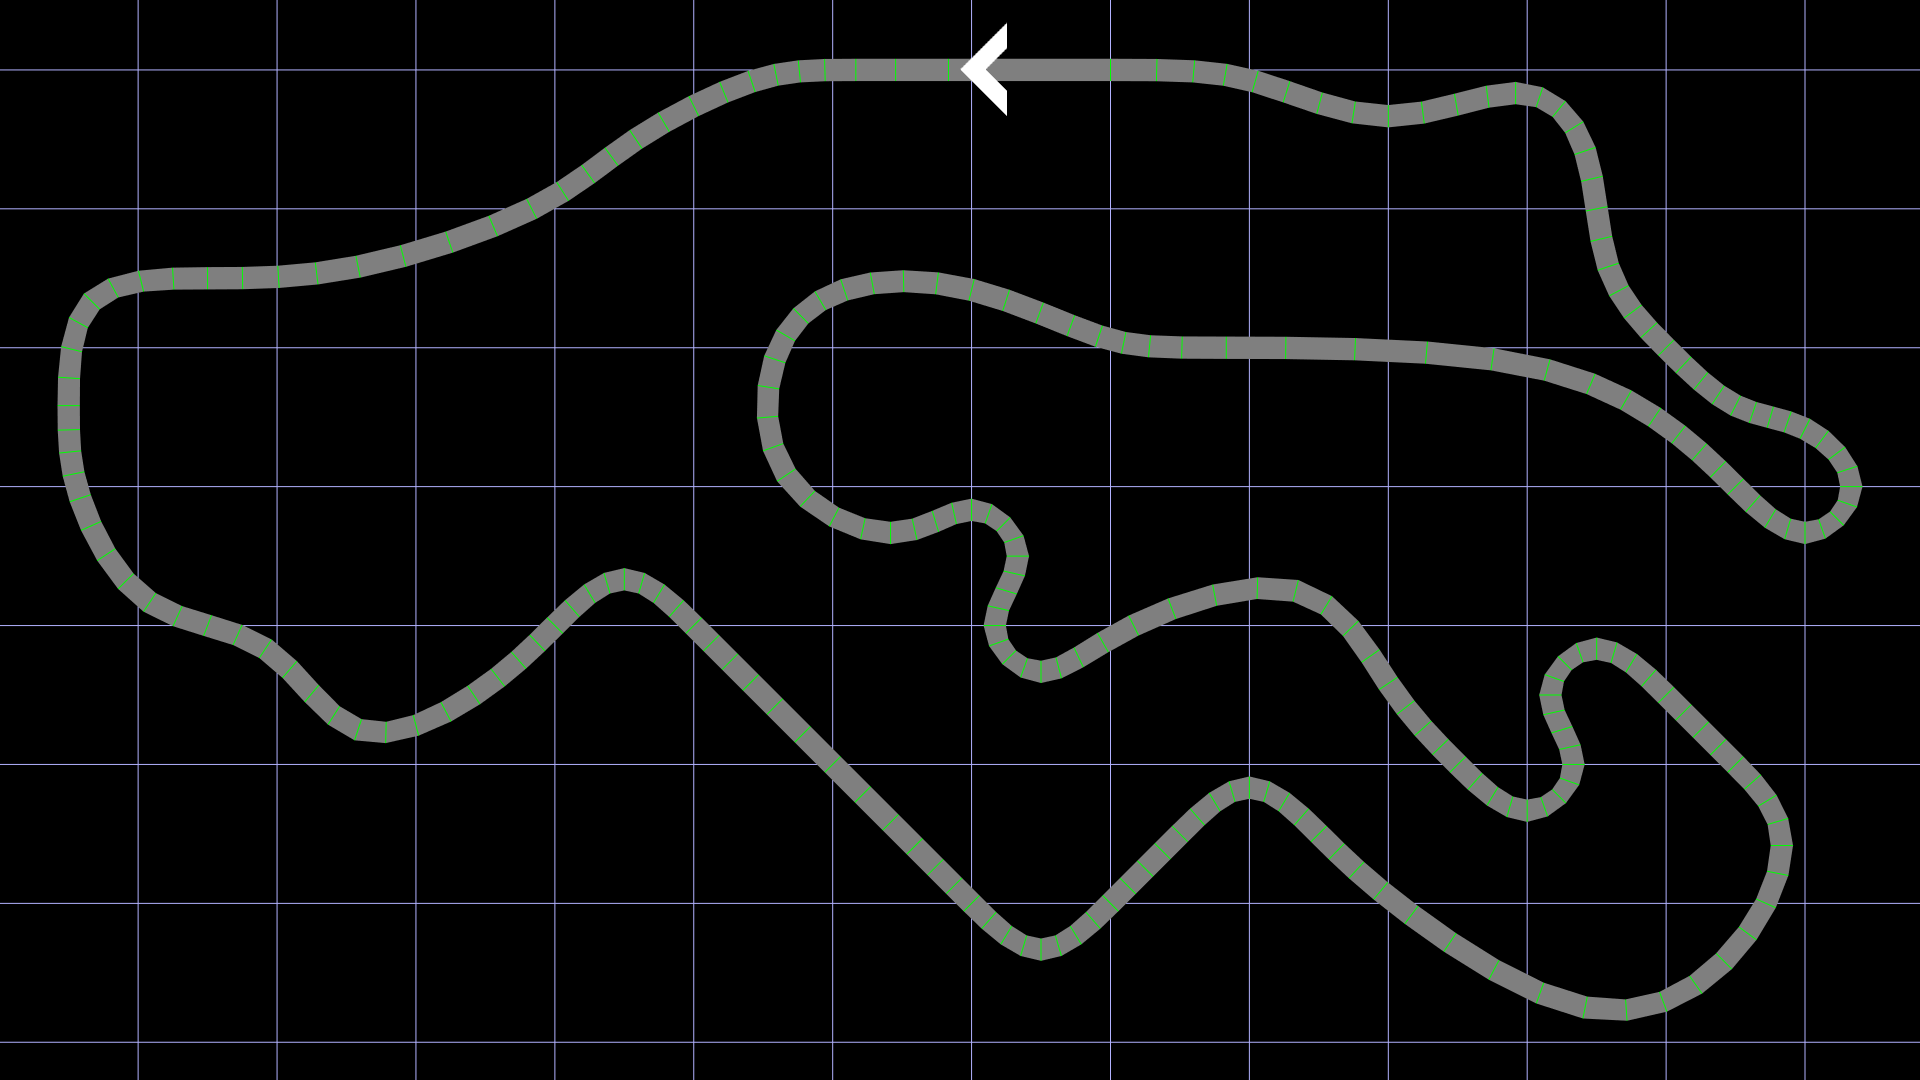
\includegraphics[width=0.45\textwidth]{mirrored}}}%
   
    \caption{The original and mirrored versions of the circuit. The arrows show the starting position and direction of the car on each track.}
    \label{fig:mirrored_tracks}
\end{figure}

\noindent
There is a wide range of possible results in this experiment, in the worst case, the performance of the trained group is equal or worse than the control group and in the best case it performs as well as before the change of circuit. The best case scenario is unlikely, since the genomes will encounter corners they have never encountered before. However, if the test population outperforms the control group in any significant way it shows that the population has acquired some general knowledge of how to turn or manage the speed. 

If the results show some form of generalisation there is a possible extension to the experiment that could yield interesting results. The extension regards the extent to which the population forgets knowledge about the original circuit when migrated. If the population is migrated back to the original track after learning how to drive on the mirrored one, will it still remember how to drive on it? Can the population learn to drive well on one track without forgetting how to drive well on the other?


